\chapter{Ingegneria del software Agile}\label{ch-02}

\lecturemeta{Capitolo originale: 2 --- Agile Software Engineering \quad\textbullet\quad Antonio Brogi}{Appunti di Emiliano Sescu (github.com/Faxatos), cap. 2}

Per circa 50 anni l'ingegneria del software è stata dominata dallo
sviluppo \textbf{plan-driven} (guidato da un piano), che prevedeva:

\begin{itemize}
\tightlist
\item
  una pianificazione dettagliata del progetto (parte molto pesante);
\item
  la specifica dei requisiti (anch'essa molto onerosa);
\item
  metodi di analisi e progettazione;
\item
  una documentazione completa del sistema;
\item
  un controllo di qualità formale.
\end{itemize}

All'inizio degli anni 2000 viene pubblicato il \textbf{Manifesto per lo
sviluppo agile del software}, che mette al primo posto:

\begin{itemize}
\tightlist
\item
  \textbf{Individui e interazioni} più che processi e strumenti.
\item
  \textbf{Software funzionante} più che documentazione esaustiva. La
  documentazione serve a chi modificherà il codice in futuro, ma
  renderla dettagliata costa molto.
\item
  \textbf{Collaborazione con il cliente} più che negoziazione del
  contratto: il cliente entra nel processo di sviluppo.
\item
  \textbf{Rispondere al cambiamento} più che seguire un piano, perché
  nessuno può prevedere il futuro.
\end{itemize}

\begin{boxnote}{``Più che'' non vuol dire ``invece di''}

Il manifesto non dice che processi, documentazione, contratti e piani
siano inutili: dice che hanno valore, ma che gli elementi a sinistra ne
hanno \textbf{di più}.

\end{boxnote}

La vera novità di Agile è smettere di pensare le applicazioni come si
faceva prima e allinearsi a come \textbf{gli utenti} vedono il sistema:
un insieme di funzionalità. Uno dei principi chiave è lo
\textbf{sviluppo incrementale}: si scelgono poche funzionalità, si
implementano, e si ripete.

\begin{figure}[H]
\centering
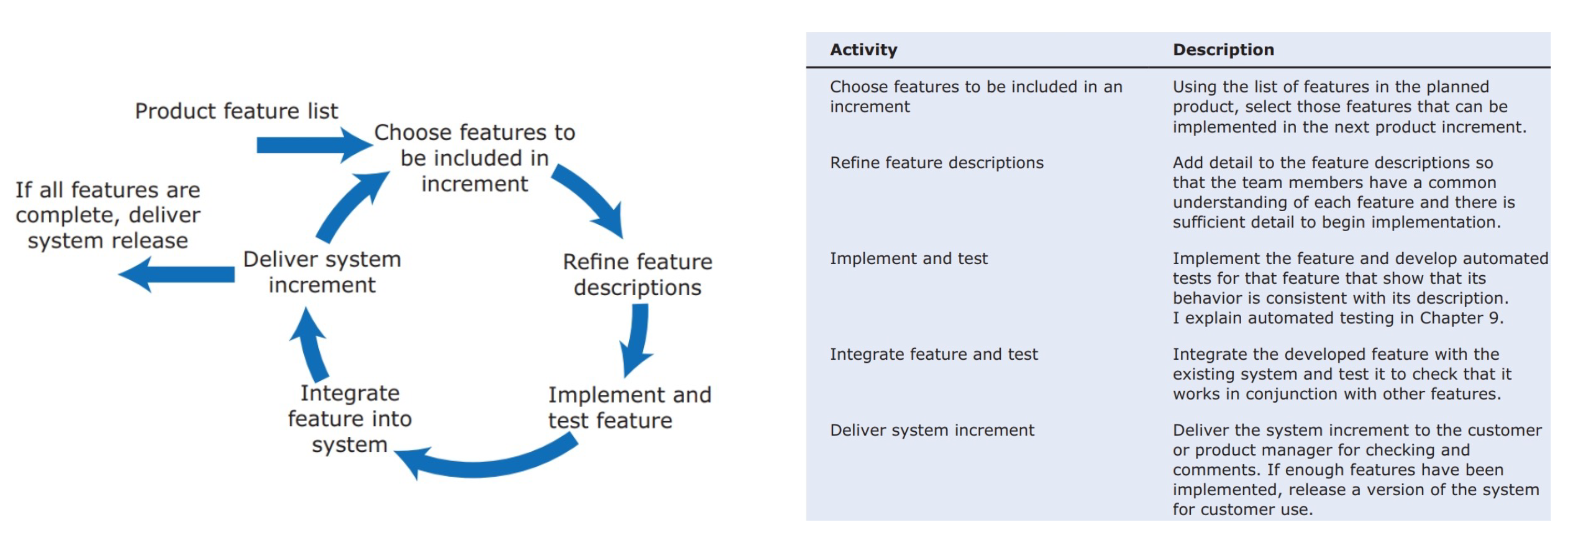
\includegraphics[width=1.00\linewidth,height=0.45\textheight,keepaspectratio]{images/02-agile_fig2-1_ciclo-incrementale.png}
\caption{Il ciclo di Continuous Integration e Continuous Deployment.}
\end{figure}

Il ciclo si ripete finché il sistema non è completo. Ogni giro può anche
fallire, perché si sono capite male le funzionalità richieste o perché
il cliente ha cambiato idea. Questo processo, che si può immaginare come
una \emph{pipeline}, si chiama \textbf{Continuous Integration e
Continuous Delivery/Deployment (CI/CD)}.

Oltre ai quattro valori, il manifesto elenca \textbf{dodici principi}
(tra parentesi il significato pratico):

\begin{enumerate}
\def\labelenumi{\arabic{enumi}.}
\tightlist
\item
  La priorità massima è \textbf{soddisfare il cliente} con consegne
  rapide e continue di software di valore (appena c'è un pezzo di
  software usabile, va rilasciato).
\item
  \textbf{I cambiamenti nei requisiti sono benvenuti}, anche a sviluppo
  avanzato: i processi agili li sfruttano come vantaggio competitivo per
  il cliente (è irrealistico avere tutte le funzionalità chiare fin
  dall'inizio: bisogna accettare che i requisiti cambino).
\item
  \textbf{Consegnare spesso software funzionante}, da ogni paio di
  settimane a ogni paio di mesi, preferendo i tempi più brevi (pipeline
  CI/CD).
\item
  Chi si occupa del business e gli sviluppatori devono \textbf{lavorare
  insieme ogni giorno} per tutto il progetto.
\item
  I progetti si costruiscono attorno a \textbf{persone motivate}:
  bisogna dare loro l'ambiente e il supporto di cui hanno bisogno e
  fidarsi di loro (principio assente negli appunti originali).
\item
  Il modo più efficace per passare informazioni al team e dentro il team
  è la \textbf{conversazione faccia a faccia}.
\item
  Il \textbf{software funzionante} è la misura principale del progresso
  (non la consegna di nuova documentazione o specifiche).
\item
  I processi agili promuovono uno \textbf{sviluppo sostenibile}:
  sponsor, sviluppatori e utenti devono poter mantenere un ritmo
  costante indefinitamente.
\item
  L'attenzione continua all'\textbf{eccellenza tecnica} e al buon design
  aumenta l'agilità.
\item
  La \textbf{semplicità}, cioè l'arte di massimizzare il lavoro
  \emph{non} fatto, è essenziale.
\item
  Le migliori architetture, requisiti e design emergono da \textbf{team
  auto-organizzati} (invece che da team separati in stanze diverse).
\item
  A intervalli regolari il team \textbf{riflette} su come diventare più
  efficace e adatta il suo comportamento di conseguenza.
\end{enumerate}

\section{Extreme Programming (XP)}\label{extreme-programming-xp}

L'\textbf{Extreme Programming (XP)} è una delle prime tecniche nate
all'interno della metodologia Agile. I suoi punti chiave sono riassunti
nell'immagine:

\begin{figure}[H]
\centering
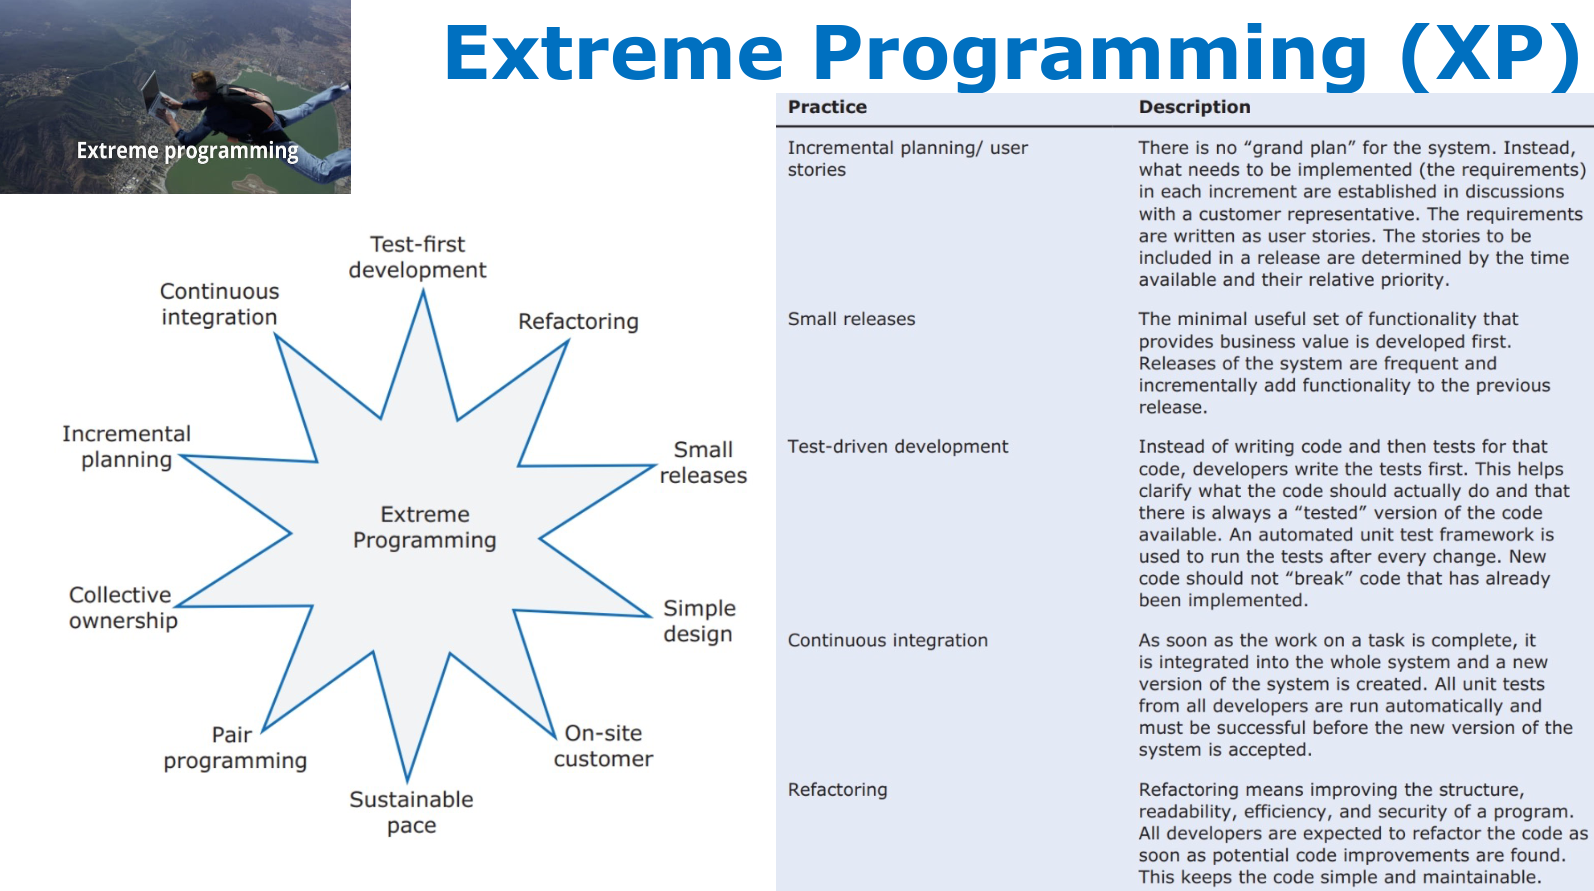
\includegraphics[width=1.00\linewidth,height=0.45\textheight,keepaspectratio]{images/02-agile_fig2-2_extreme-programming.png}
\caption{I principi dell'Extreme Programming.}
\end{figure}

Le pratiche descritte nella tabella della figura sono:

\begin{itemize}
\tightlist
\item
  \textbf{Incremental planning / user stories}: non c'è un ``grande
  piano''. Cosa implementare in ogni incremento si decide con un
  rappresentante del cliente, scrivendo i requisiti come \emph{user
  story}; le storie da includere in una release dipendono dal tempo
  disponibile e dalla loro priorità.
\item
  \textbf{Small releases}: si parte dall'insieme minimo di funzionalità
  utile che porta valore, e le release successive, frequenti, aggiungono
  funzionalità un po' alla volta.
\item
  \textbf{Test-driven development}: prima di scrivere il codice si
  scrivono i test per quella funzionalità. Questo chiarisce cosa deve
  fare il codice e fa sì che ci sia sempre una versione ``testata'' del
  codice. Un framework di test automatici controlla che il nuovo codice
  non rompa quello esistente.
\item
  \textbf{Continuous integration}: appena un compito è finito, viene
  integrato nel sistema completo e si crea una nuova versione; tutti i
  test di unità devono passare prima che la nuova versione sia
  accettata.
\item
  \textbf{Refactoring}: migliorare struttura, leggibilità, efficienza e
  sicurezza del programma. Tutti gli sviluppatori devono fare
  refactoring appena trovano possibili miglioramenti, per mantenere il
  codice semplice e manutenibile.
\end{itemize}

\section{Scrum}\label{scrum}

\begin{boxdefinition}{Scrum}

\textbf{Scrum} è un framework leggero che aiuta persone, team e
organizzazioni a generare valore attraverso soluzioni adattive a
problemi complessi. Contiene un insieme di principi e regole da seguire
per raggiungere un obiettivo comune.

\end{boxdefinition}

La motivazione è questa: i manager di un'azienda software hanno bisogno
di sapere quanto costerà sviluppare un prodotto, quanto tempo servirà e
quando potrà uscire sul mercato. Lo sviluppo plan-driven risponde con
piani di lungo periodo che indicano i \textbf{deliverable} (cosa il team
consegnerà e quando). Però i piani cambiano sempre: sono affidabili solo
quelli di breve periodo.

Scrum si basa su due idee:

\begin{itemize}
\tightlist
\item
  l'\textbf{empirismo}: la conoscenza viene dall'esperienza e le
  decisioni si prendono in base a ciò che si osserva;
\item
  il \textbf{pensiero Lean}: ridurre gli sprechi e concentrarsi
  sull'essenziale.
\end{itemize}

Usa un approccio \textbf{iterativo e incrementale} per rendere il lavoro
più prevedibile e controllare il rischio. I tre \textbf{pilastri} di
Scrum sono:

\begin{itemize}
\tightlist
\item
  \textbf{Trasparenza}: l'avanzamento e il lavoro devono essere visibili
  sia a chi li svolge sia a chi li riceve.
\item
  \textbf{Ispezione}: gli artefatti di Scrum e i progressi verso gli
  obiettivi concordati vanno controllati spesso e con attenzione, per
  scoprire problemi o deviazioni indesiderate.
\item
  \textbf{Adattamento}: se qualcosa nel processo si discosta oltre i
  limiti accettabili (es. nuovi requisiti) o il prodotto non va bene,
  bisogna correggere il processo o ciò che si sta producendo, e farlo il
  prima possibile.
\end{itemize}

Scrum funziona se le persone vivono i suoi \textbf{cinque valori}:
\textbf{Impegno} (\emph{commitment}, rispettare le scadenze),
\textbf{Focus}, \textbf{Apertura} (verso nuove soluzioni),
\textbf{Rispetto} (per i compagni di team e gli altri) e
\textbf{Coraggio} (di proporre soluzioni che allineino meglio il
prodotto alla sua visione).

\subsection{Scrum Team}\label{scrum-team}

Un team \textbf{auto-organizzato} coordina il lavoro discutendo i
compiti e decidendo insieme chi fa cosa. Il team decide da solo tempi e
deliverable, e gli sviluppatori sono coinvolti il meno possibile nelle
\textbf{interazioni esterne}, cioè quelle con persone fuori dal team
(management e clienti). L'idea di Scrum è che gli sviluppatori pensino
solo a sviluppare: le interazioni esterne le gestiscono \textbf{Scrum
Master} e \textbf{Product Owner}, così il team lavora senza interferenze
o distrazioni.

\subsubsection{Product Owner}\label{product-owner}

Il \textbf{Product Owner} fa in modo che il team resti concentrato sulla
costruzione del prodotto, senza perdersi in lavori tecnicamente
interessanti ma poco rilevanti. Nello sviluppo di prodotti, di solito
questo ruolo lo ricopre il Product Manager.

\begin{boxtip}{Chi gestisce cosa}

Le interazioni esterne \textbf{legate al prodotto} le gestisce il
\textbf{Product Owner}.

\end{boxtip}

\subsubsection{Scrum Master}\label{scrum-master}

Lo \textbf{Scrum Master} è un esperto di Scrum che guida il team
nell'usare bene il metodo. Non è un project manager tradizionale ma un
\textbf{coach} del team, con autorità su \emph{come} il team usa Scrum.
In molte aziende però si occupa anche di parte della gestione del
progetto.

Il motivo è pratico: tranne che nelle aziende molto piccole, il team
deve riferire i progressi al management, e qualcuno deve farlo. Ruotare
questo compito tra i membri non funziona, perché serve continuità nei
rapporti con l'esterno. Lo Scrum Master è la persona che conosce meglio
lo stato del lavoro, quindi è quella più adatta a fornire informazioni e
piani affidabili, anche se gli ideatori di Scrum non l'avevano previsto.

\begin{boxtip}{Chi gestisce cosa}

Le interazioni esterne \textbf{legate al team} le gestisce lo
\textbf{Scrum Master}.

\end{boxtip}

\subsubsection{Developers}\label{developers}

I team auto-organizzati prendono le decisioni discutendo e trovando un
accordo. La \textbf{dimensione ideale} di un team Scrum è di \textbf{5-8
persone}: abbastanza per avere competenze diverse (reti, user
experience, database, \ldots) e livelli di esperienza diversi, ma
abbastanza poche per comunicare in modo informale ed efficace e mettersi
d'accordo sulle priorità.

Il vantaggio di un team auto-organizzato è che diventa coeso e si adatta
ai cambiamenti. Visto che la responsabilità del lavoro è del team e non
dei singoli, il team regge anche l'uscita o l'ingresso di persone.
Inoltre, comunicando molto, i membri imparano a conoscere le competenze
degli altri.

Scrum assume che il team lavori nello \textbf{stesso spazio} e che il
\textbf{daily scrum} (la riunione quotidiana) tenga tutti aggiornati. Ma
due ipotesi dietro il daily scrum non sempre valgono:

\begin{itemize}
\tightlist
\item
  Scrum assume persone a tempo pieno nello stesso ufficio. In realtà si
  può lavorare part-time o da luoghi diversi (e, in un team di studenti,
  ognuno segue lezioni in orari diversi).
\item
  Scrum assume che tutti possano partecipare a una riunione mattutina.
  In realtà qualcuno ha orari flessibili (es. per impegni familiari) o
  lavora a più progetti contemporaneamente.
\end{itemize}

\subsection{Artefatti}\label{artefatti}

\subsubsection{Product Backlog}\label{product-backlog}

\begin{boxdefinition}{Product backlog}

Il \textbf{product backlog} è la lista delle cose da fare per sviluppare
il prodotto. Viene rivisto e aggiornato prima di ogni sprint.

\end{boxdefinition}

\begin{figure}[H]
\centering
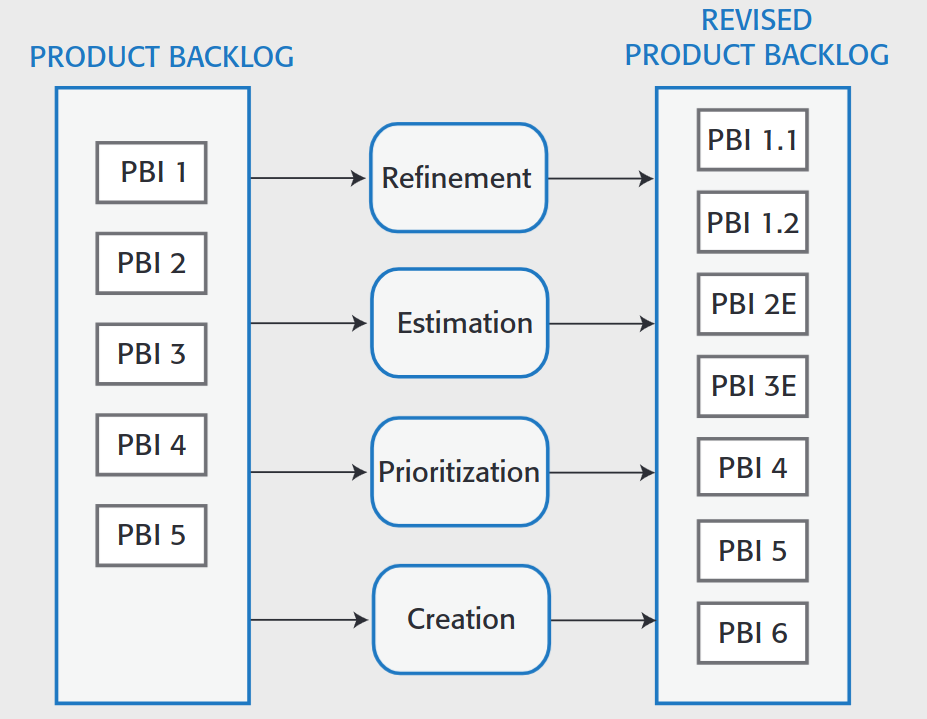
\includegraphics[width=0.80\linewidth,height=0.45\textheight,keepaspectratio]{images/02-agile_fig2-3_product-backlog.png}
\caption{Il product backlog durante le attività sul backlog.}
\end{figure}

Come mostra la figura, gli elementi (\textbf{PBI}, \emph{Product Backlog
Item}) vengono prima selezionati e messi in ordine di priorità; in base
alla priorità verranno implementati nello sprint successivo. Alcuni
esempi di PBI:

\begin{itemize}
\tightlist
\item
  ``Come insegnante, voglio poter configurare gli strumenti disponibili
  per ogni classe.'' (\emph{feature})
\item
  ``Come genitore, voglio poter vedere i lavori dei miei figli e le
  valutazioni degli insegnanti.'' (\emph{feature})
\item
  ``Come insegnante di bambini piccoli, voglio un'interfaccia a immagini
  per chi non sa ancora leggere bene.'' (\emph{richiesta di un utente})
\item
  ``Cifrare tutti i dati personali degli utenti.'' (\emph{miglioramento
  tecnico})
\end{itemize}

Un PBI può trovarsi in tre \textbf{stati}:

\begin{itemize}
\tightlist
\item
  \textbf{Ready for consideration}: idee e descrizioni di feature ad
  alto livello, ancora in valutazione. Sono provvisorie: possono
  cambiare o non entrare mai nel prodotto.
\item
  \textbf{Ready for refinement}: il team è d'accordo che l'elemento è
  importante e va fatto nel ciclo corrente. Cosa serve è abbastanza
  chiaro, ma va ancora raffinato.
\item
  \textbf{Ready for implementation}: il PBI è abbastanza dettagliato da
  poter stimare lo sforzo e iniziare a implementarlo. Sono note anche le
  dipendenze da altri elementi.
\end{itemize}

\subsubsection{Sprint Backlog}\label{sprint-backlog}

\begin{boxdefinition}{Sprint backlog}

Lo \textbf{sprint backlog} è la lista ristretta di compiti, presi dal
product backlog, che il team si impegna a completare durante lo sprint.

\end{boxdefinition}

Si crea durante lo \emph{sprint planning}: si scelgono gli elementi in
base all'obiettivo dello sprint e li si divide in compiti più piccoli e
concreti. A differenza del product backlog, che contiene tutte le
possibili feature e migliorie, lo sprint backlog contiene \textbf{solo
ciò che si può fare nel tempo dello sprint}. Durante lo sprint il team
lo aggiorna per segnare i compiti completati e i cambiamenti.

Lo sprint backlog aiuta il team a restare allineato all'obiettivo e a
gestire l'avanzamento. Per visualizzare il lavoro e il tempo rimanenti
si usano spesso i \textbf{burn-down chart}.

\subsection{Eventi Scrum}\label{eventi-scrum}

In Scrum il software si sviluppa in periodi di durata fissa chiamati
\textbf{sprint}, di solito lunghi \textbf{2-4 settimane}. Durante lo
sprint il team fa riunioni quotidiane (gli \emph{scrum}) per controllare
l'avanzamento e aggiornare la lista del lavoro ancora da fare. Ogni
sprint deve produrre un \textbf{incremento di prodotto rilasciabile}
(\emph{shippable product increment}): il software sviluppato deve essere
completo e pronto per il deploy.

Gli sprint sono \textbf{timeboxed}: lo sviluppo si ferma alla fine dello
sprint, che il lavoro sia finito o no.

Le attività di uno sprint sono tre:

\begin{itemize}
\tightlist
\item
  \textbf{Sprint Planning}: il team sceglie gli elementi da completare
  nello sprint e, se serve, li raffina per creare lo sprint backlog. Non
  dovrebbe durare più di un giorno, all'inizio dello sprint.
\item
  \textbf{Sprint Execution}: il team implementa gli elementi dello
  sprint backlog. Se non riesce a completarli tutti, lo sprint
  \textbf{non viene allungato}: gli elementi non finiti tornano nel
  product backlog per gli sprint successivi.
\item
  \textbf{Sprint Review}: il team (ed eventualmente stakeholder esterni)
  rivede il lavoro fatto, ragionando su cosa è andato bene, cosa è
  andato male e come migliorare il processo.
\end{itemize}

\begin{figure}[H]
\centering
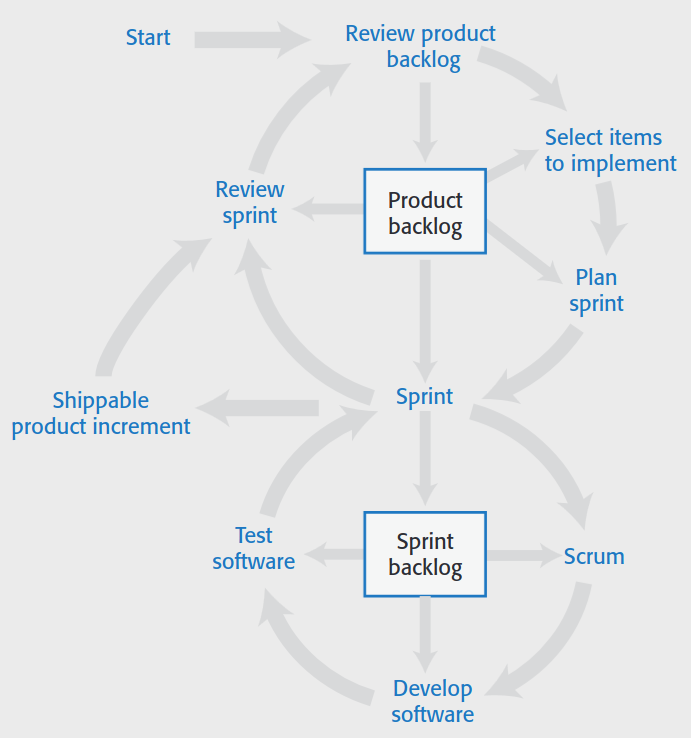
\includegraphics[width=0.70\linewidth,height=0.45\textheight,keepaspectratio]{images/02-agile_fig2-4_ciclo-scrum.png}
\caption{Le attività dello sprint all'interno del ciclo Scrum.}
\end{figure}

\subsubsection{Sprint Planning}\label{sprint-planning}

Nello sprint planning si concorda un \textbf{obiettivo dello sprint}
(\emph{sprint goal}), che può riguardare funzionalità, supporto,
prestazioni o affidabilità. Per definirlo il team sceglie quali elementi
del product backlog implementare. Il risultato è lo \textbf{sprint
backlog}, una versione più dettagliata del product backlog con i compiti
da svolgere nello sprint.

Durante lo sprint il team fa ogni giorno un \textbf{daily scrum} per
coordinarsi: una riunione breve, di solito a inizio giornata, in cui
ognuno racconta cosa ha fatto, che problemi ha incontrato e cosa farà
oggi. Così tutti sanno cosa succede e si può ripianificare in fretta se
serve.

\begin{boxtip}{Stand-up meeting}

Gli scrum devono restare brevi e concentrati. Per evitare discussioni
lunghe a volte si fanno \textbf{in piedi}, senza sedie (\emph{stand-up
meeting}).

\end{boxtip}

Durante lo scrum si rivede lo sprint backlog: si tolgono gli elementi
completati e se ne aggiungono di nuovi se emergono nuove informazioni.
Poi il team decide chi lavora su cosa quel giorno.

\subsubsection{Sprint Execution}\label{sprint-execution}

Scrum non impone pratiche tecniche specifiche durante lo sprint, ma due
sono molto consigliate:

\begin{itemize}
\tightlist
\item
  \textbf{Test automation}: automatizzare più test possibile, creando
  una suite di test eseguibili in qualsiasi momento per controllare la
  qualità del software.
\item
  \textbf{Continuous Integration}: ogni volta che si modifica un
  componente, lo si integra subito con gli altri per ottenere il sistema
  completo, che poi si testa per scoprire problemi imprevisti nelle
  interazioni tra componenti.
\end{itemize}

\subsubsection{Sprint Review}\label{sprint-review}

Alla fine di ogni sprint c'è una \textbf{sprint review} con tutto il
team. Si controlla se l'obiettivo dello sprint è stato raggiunto, si
discutono i problemi nuovi emersi e si ragiona su come migliorare il
modo di lavorare.

È il \textbf{Product Owner} a decidere se l'obiettivo è stato raggiunto,
confermando che gli elementi scelti sono stati implementati
completamente. La review include anche una \textbf{revisione del
processo}: il team riflette su come ha usato Scrum e su come essere più
produttivo nello sprint successivo.

\subsection{Esecuzione: le attività sul
backlog}\label{esecuzione-le-attivituxe0-sul-backlog}

A seconda dello stato di un PBI si possono fare diverse azioni:

\begin{itemize}
\tightlist
\item
  \textbf{Refinement} (raffinamento): si analizzano i PBI esistenti e li
  si divide in PBI più dettagliati. Può portare alla creazione di nuovi
  elementi.
\item
  \textbf{Estimation} (stima): il team stima quanto lavoro serve per
  implementare un PBI e aggiunge la stima al PBI.
\item
  \textbf{Creation} (creazione): si aggiungono nuovi elementi al
  backlog, ad esempio feature proposte dal product manager, modifiche a
  feature esistenti, miglioramenti tecnici o attività di processo (come
  valutare nuovi strumenti di sviluppo).
\item
  \textbf{Prioritization} (priorità): i nuovi elementi vengono ordinati
  per priorità all'interno del backlog.
\end{itemize}

Gli effetti di queste azioni si vedono in Fig. 2.3. Per decidere lo
stato o l'azione successiva di un PBI si usano alcune metriche:

\begin{itemize}
\tightlist
\item
  \textbf{Sforzo richiesto} (\emph{effort}): in persone-ora o
  persone-giorno, cioè le ore o i giorni che servirebbero a \textbf{una}
  persona per implementare il PBI. Non coincide con il tempo di
  calendario, perché più persone possono lavorare sullo stesso elemento.
\item
  \textbf{Story point}: una stima arbitraria dello sforzo che tiene
  conto di dimensione del compito, complessità, tecnologie necessarie e
  parti ``sconosciute'' del lavoro. Nascono dal confronto tra user story
  ma si possono usare per qualsiasi PBI. Si stimano in modo
  \textbf{relativo}: il team fissa i punti di un compito di riferimento
  e stima gli altri per confronto (più/meno complesso, più grande/più
  piccolo, \ldots).
\end{itemize}

\begin{boxexample}{Sforzo vs tempo di calendario}

Un PBI stimato 10 persone-giorno, se ci lavorano in due, può essere
finito in circa 5 giorni di calendario.

\end{boxexample}
